\chapter{Introduction}
\label{chpt:intro}

Advances in deep neural networks have opened a new era of robotics, intelligent robots. Compared with traditional robots that perform repetitive tasks based on manual control or predefined rules, intelligent robots possess a more comprehensive perception of environments and make more sophisticated decisions for various tasks \citep{wang2018current}.

On the other hand, the development of physics engines and realistic renderers makes it feasible to simulate complex robots in simulators. Reinforcement learning that learns from trial and error, can now be trained and verified in a virtual environment before deploying to the physical world.

However, recent research unveils that deep neural networks are vulnerable to adversarial attacks, including deep reinforcement learning. This research intends to design more robust and accountable autonomous systems so that we can safely embrace the benefit of deep learning.


\section{Intelligent Robots}
\label{sec:intelligent_robot}

The upsurge of cloud service, deep learning for computer vision, natural language processing,  and etc empowers robots to have more interactions with humans, and other robots. 

\begin{figure}[H]
\centering
\begin{subfigure}[b]{0.485\textwidth}
    \centering
    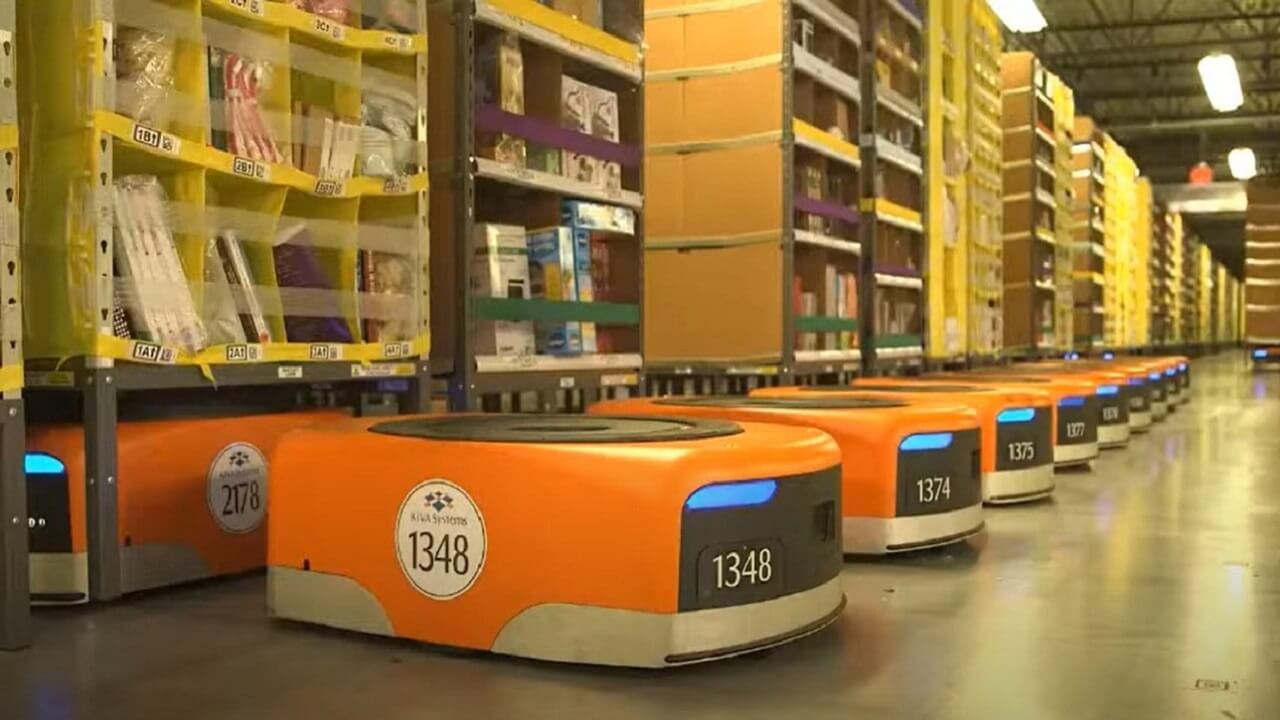
\includegraphics[width=\textwidth]{figures/chapter_intro/amazon_kiva.jpg}
    \caption{Amazon Kiva Robot}
    \label{fig:kiva}
\end{subfigure}
\hfill
\begin{subfigure}[b]{0.485\textwidth}
    \centering
    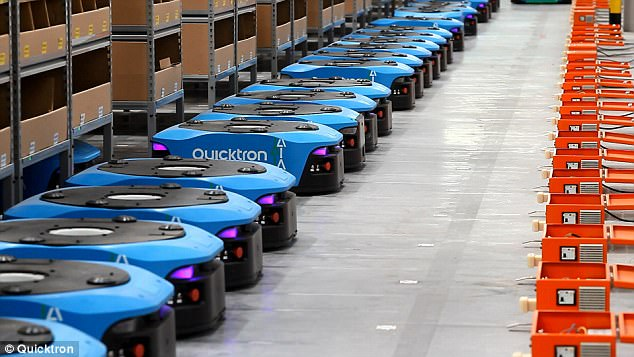
\includegraphics[width=\textwidth]{figures/chapter_intro/alibaba_quicktron.jpg}
    \caption{Alibaba Quicktron Robot}
    \label{fig:quicktron}
\end{subfigure}
\hfill
\caption{Robots in warehouse.}
\label{fig.robot}
\end{figure}

For instance, the Amazon Kiva Robot and Alibaba Quicktron Robot can help warehouse staffs find desired items by moving goods shelves. Each robot can perceive the surrounding environment to avoid collisions with other robots, and receive commands from warehouse staff via cloud servers. On the other hand, autonomous driving research teams from Waymo (formerly the Google self-driving car project), Tesla, etc intend to achieve autonomous navigation without human interference.

\begin{figure}[H]
\centering
\begin{subfigure}[b]{0.485\textwidth}
    \centering
    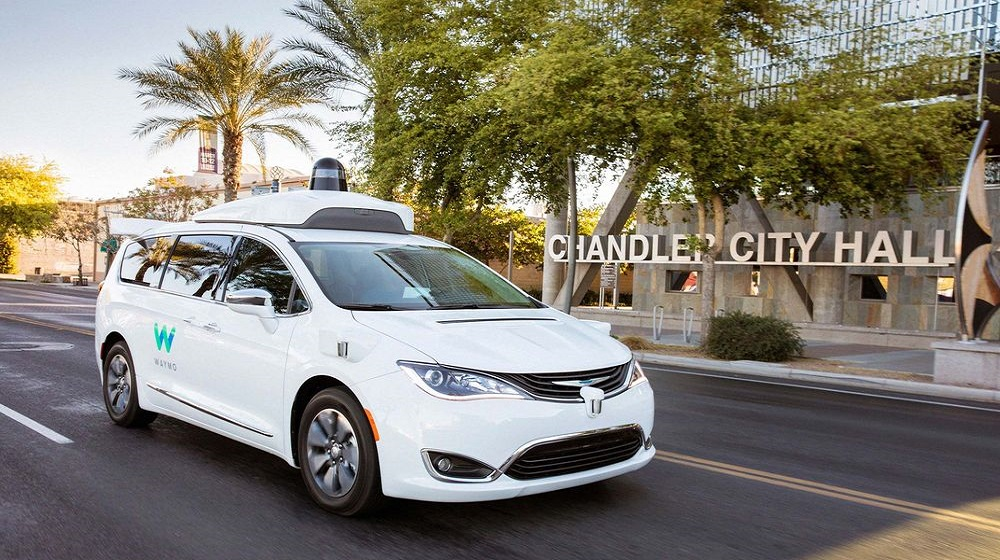
\includegraphics[width=\textwidth]{figures/chapter_intro/waymo.jpg}
    \caption{Waymo (formerly Google self-driving project)}
    \label{fig:waymo}
\end{subfigure}
\hfill
\begin{subfigure}[b]{0.485\textwidth}
    \centering
    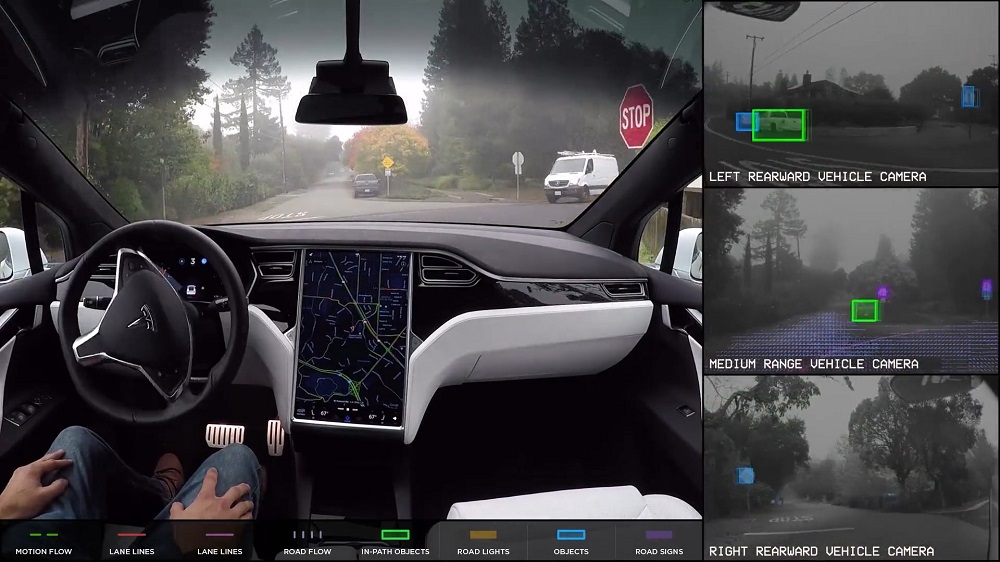
\includegraphics[width=\textwidth]{figures/chapter_intro/tesla_autopilot.jpg}
    \caption{Tesla Autopilot}
    \label{fig:tesla}
\end{subfigure}
\hfill
\caption{Autonomous Driving Research}
\label{fig.autonomous}
\end{figure}

Autonomous driving systems are commonly divided into sub-tasks: localization, perception, prediction, planning, and control. The vehicle determines its position in the environment through localization. Perception enables vehicles to collect information and extract relevant knowledge from the environment. The task of prediction makes predictions of measurement, behavior, trajectory, etc. The planning task makes purposeful decisions to achieve the goal, and the control component executes the planned actions \citep{pendleton2017perception}. Recently, the end-to-end driving that maps inputs directly to steering commands started to rise as an alternative to modular systems.

Our research focuses on adversarial attacks against deep learning models for mobile robots perception, such as image classification, object detection and object tracking in autonomous driving. We also investigate possible vulnerabilities in deep reinforcement learning.


\subsection{Deep Learning}
\label{sec:deep_robot}

As the research in deep neural networks advances, deep convolutional networks become feasible for automated driving tasks. Our research investigates the effect of adversarial attacks against deep learning models. However, it is risky to perform attacks against real-world autonomous driving systems. Thus adversarial attacks are tested in various simulators.

\begin{figure}[H]
\centering
\begin{subfigure}[b]{0.485\textwidth}
    \centering
    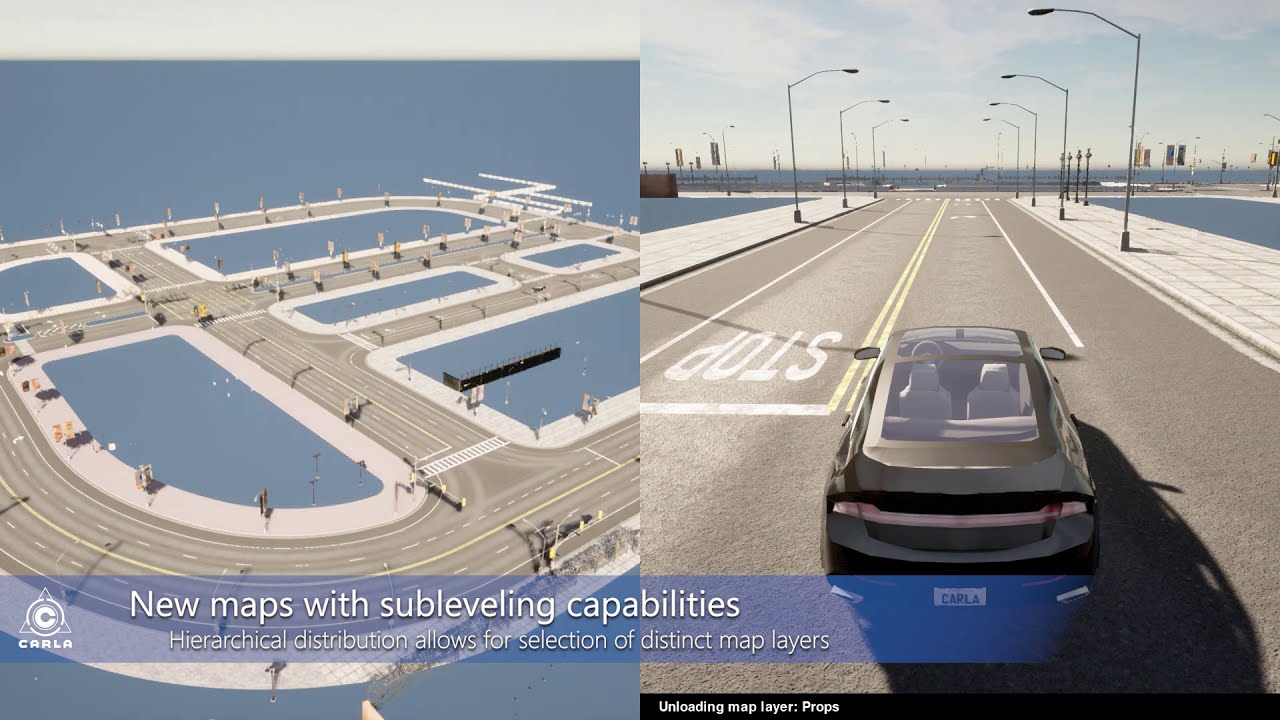
\includegraphics[width=\textwidth]{figures/chapter_intro/carla.jpg}
    \caption{Carla}
    \label{fig:carla_intro}
\end{subfigure}
\hfill
\begin{subfigure}[b]{0.485\textwidth}
    \centering
    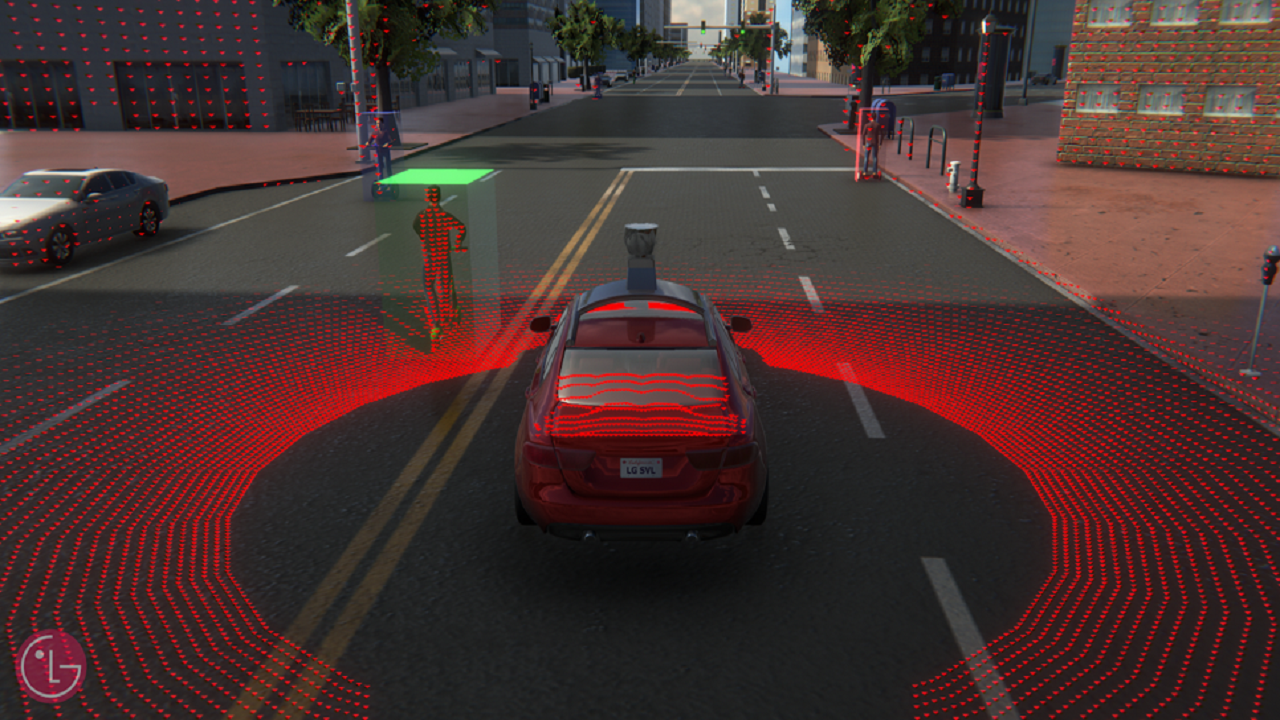
\includegraphics[width=\textwidth]{figures/chapter_intro/lgsvl.png}
    \caption{LGSVL}
    \label{fig:lvsvl}
\end{subfigure}
\hfill
\caption{Autonomous Driving Simulators}
\label{fig.simulator}
\end{figure}

The Carla simulator is an open-source platform for autonomous driving simulation based on the Unreal Game Engine. It simulates various sensors such as depth camera, 3D lidar, radar. The Carla simulator provides flexible Python API to manipulate the virtual environments and supports Robot Operating System (ROS) integration as well \citep{Dosovitskiy17}.

The LGSVL is another autonomous vehicle simulation platform based on the Unity3D Game Engine. It provides integration with the Baidu Apollo Platform \citep{rong2020lgsvl}. Besides, the Microsoft Airsim simulator provides virtual environments for both autonomous driving and drone simulation \citep{airsim2017fsr}.

\begin{figure}[H]
\centering
\begin{subfigure}[b]{0.485\textwidth}
    \centering
    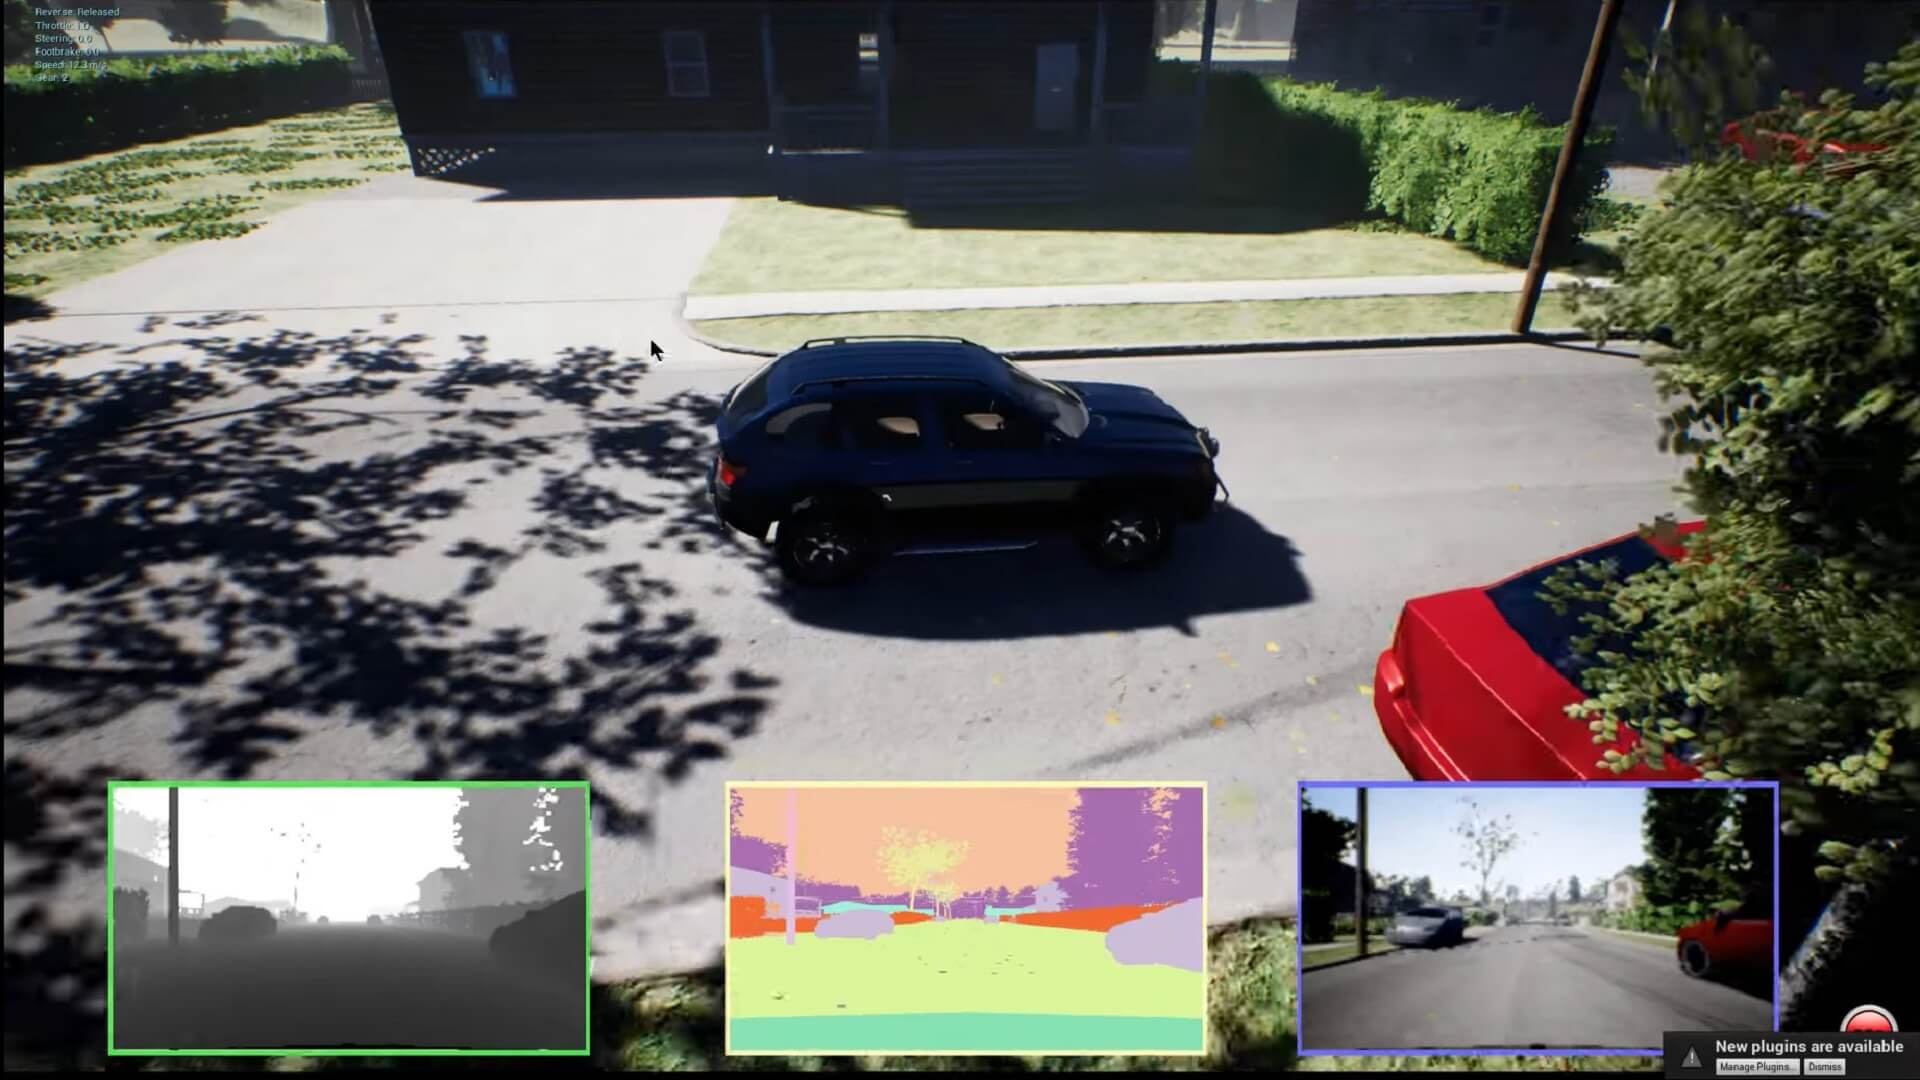
\includegraphics[width=\textwidth]{figures/chapter_intro/airsim_car.jpg}
    \caption{Airsim for Autonomous Driving}
    \label{fig:airsim_car}
\end{subfigure}
\hfill
\begin{subfigure}[b]{0.485\textwidth}
    \centering
    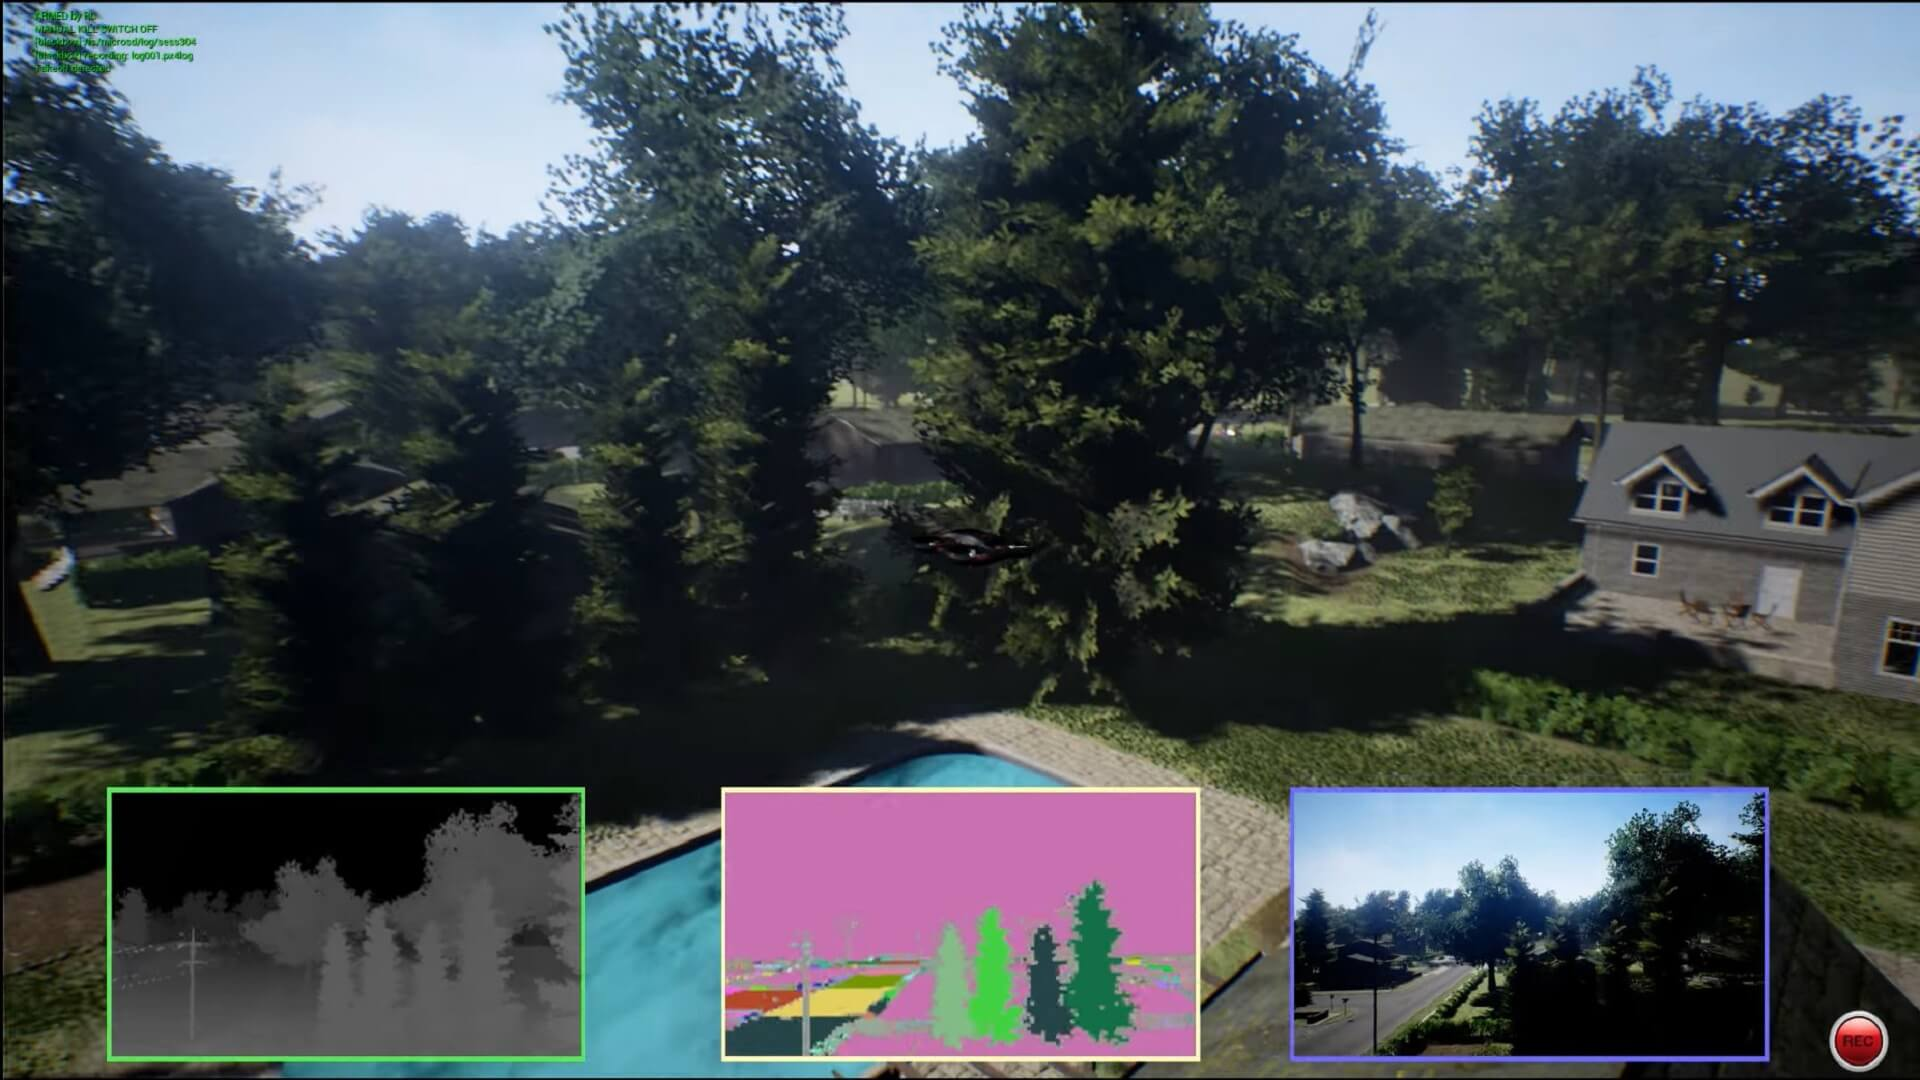
\includegraphics[width=\textwidth]{figures/chapter_intro/airsim_drone.jpg}
    \caption{Airsim for drones}
    \label{fig:airsim_drone}
\end{subfigure}
\hfill
\caption{Microsoft Airsim Simulator}
\label{fig.airsim}
\end{figure}

Practical adversarial attacks are introduced in the following three chapters. In chapter \ref{chpt:classification}, we investigate distributed black-box attacks against image classification models. In chapter \ref{chpt:detection}, we achieve real-time white-box attacks against object detection models. In chapter \ref{chpt:tracking}, we intend to attack object tracking systems, and examine the effect of hardware acceleration on the robustness of deep learning models. 

% Since end-to-end deep learning models are computationally expensive, pruning and quantization are commonly used techniques to make large models feasible for embedded systems, but theses techniques could render deep learning models more vulnerable.

In chapter \ref{chpt:defence}, the interpretability of deep learning models and defense methods against adversarial attacks are explored to help robots embrace deep neural networks safely.

% \clearpage

\subsection{Reinforcement Learning}
\label{sec:reinf_robot}

Deep reinforcement learning can be integrated into robotic systems as well. Given observations of the environment under certain states, the agent (robot) takes actions to achieve objectives. Most reinforcement learning tasks are evaluated in games such as the Atari. Recently, the NVIDIA Issac Gym simulator makes large-scale reinforcement learning possible.

\begin{figure}[H]
\centering
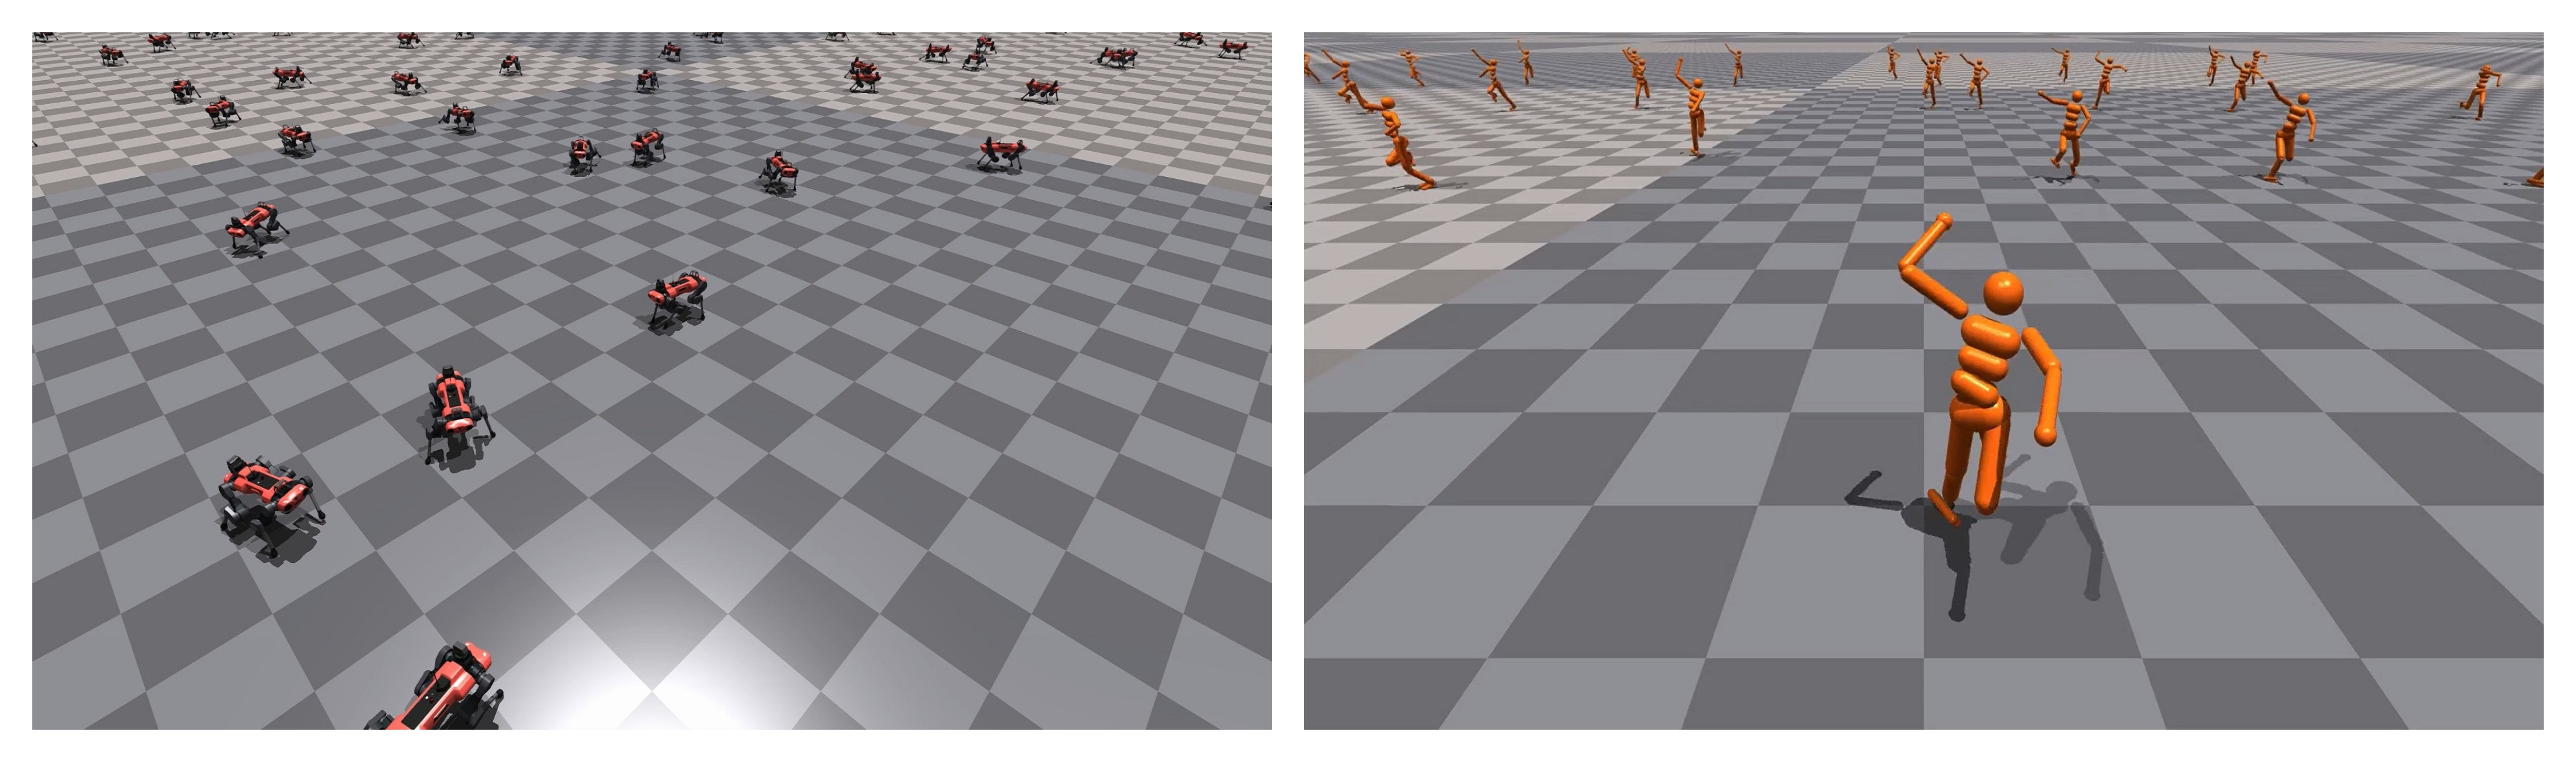
\includegraphics[width=\textwidth]{figures/chapter_intro/issac_gym.jpg}
\caption{NVIDIA Isaac Gym}
\label{fig.issac_gym}
\end{figure}

However, reinforcement learning models are vulnerable to adversarial attacks by adding perturbations to agents' observations \citep{chen2019adversarial}. Besides, recent research unveils that adversarial policy that acts abnormally in a shared environment can also induce extremely unlikely activations to occur.

\begin{figure}[H]
\centering
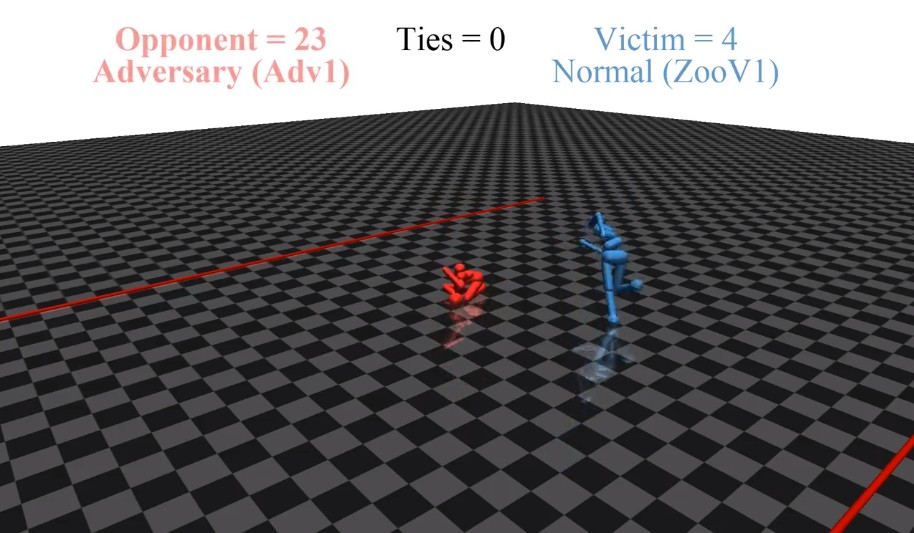
\includegraphics[scale=0.4]{figures/chapter_intro/adv_policy.jpg}
\caption{Adversarial Policies: Attacking Deep Reinforcement Learning}
\label{fig.adv_policy}
\end{figure}

For instance, the red agent tries to prevent the blue agent from crossing the line. Unexpectedly, the red agent wins the game by falling to the ground, which looks like a random policy. But this abnormal action of the red agent effectively causes the blue agent to fall as well \citep{gleave2021adversarial}. 

In chapter \ref{chpt:driving}, we provide more experiments of adversarial attacks against end-to-end models in autonomous driving systems.

\section{Adversarial Attacks}
\label{sec:adv_attack}

Existing adversarial attacks can be categorized into white-box, gray-box, and black-box attacks \citep{REN2020346}. In white-box attacks, the adversaries have full knowledge of the target model, including model architecture and parameters \citep{goodfellow2015explaining}. In gray-box attacks, the adversaries only have access to the structure of the target model. In black-box attacks, the adversaries can only gather information about the model through querying. In our research, we majorly focus on white-box and black-box attacks.

Depending on the goal of the attack, adversarial attacks can be further categorized into three types, evasion, poisoning, and extraction attacks \citep{art2018}. Evasion attacks cause models to make incorrect predictions by adding perturbations to the input during inference. The poisoning attack injects malicious data into the training set. Lastly, the extraction attack steals or replicates models that are available to query. For autonomous systems, rather than trying to steal models or poison others' training data, we intend to design a system that is resistant to malicious perturbations in the input. Thus our research object coincides with evasion attacks.

\subsection{White-Box Attacks}
\label{sec:whitebox_attack}

Deep learning models are trained by minimizing the loss function via updating weights according to gradients, while white-box attacks maximize the loss function by adding noises to the input.

\begin{figure}[H]
\centering
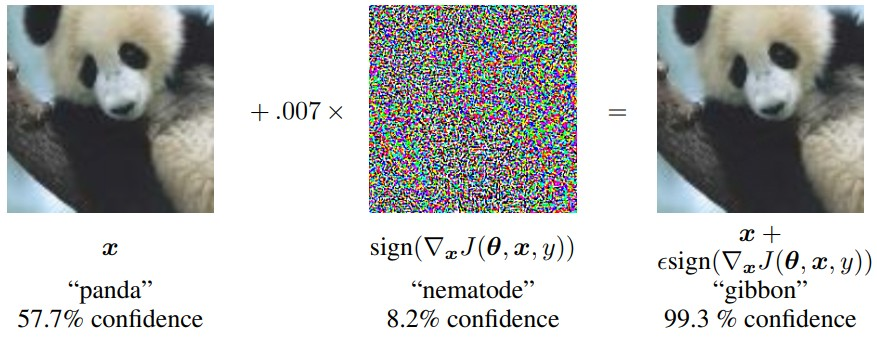
\includegraphics[scale=0.5]{figures/chapter_intro/fgsm.jpg}
\caption{Unperceivable perturbations on the full image}
\label{fig.adv_perturb}
\end{figure}

White-box attacks rely on gradients to fool deep learning models. Difference attack methods use different strategies to update the input using gradients. We can either generate human-unperceivable perturbations on the full image or a human-perceivable patch on a part of the image.

Most existing research on adversarial attacks choose a classification model as the target. A neural network is denoted as $f(\cdot)$ with input $x$ and prediction $f(x)$. The corresponding optimization loss is denoted by $J(\theta, x, y)$, where $\theta$ represents the model weights. An adversarial input $x'$ is close to the original input $x$ under a specific distance metric while $f(x') \neq f(x)$ \citep{REN2020346}. Formally, an adversarial sample of  is defined as follows:

$$x': D(x, x') < \eta, f(x') \neq y $$

Where $D(\cdot, \cdot)$ is the distance metric and $ \eta $ is a predefined distance constraint that defines the maximum allowed perturbation. The most commonly used distance metric is the $L_p$ distance metric. The distance between $x$ and $x'$ is denoted as $||x-x'||_{p}$, where $||\cdot||_p$ is defined as follows:

$$ ||v||_p = (|v_1|^p + |v_2|^p + \dots + |v_d|^p)^{1/p} $$

Where $p$ is a real number; $d$ is the dimension of the distance vector $v$. For instance, the $L_0$ distance corresponds to the number of pixels being modified in the perturbation. The $L_2$ distance measures the standard Euclidean distance between $x$ and $x'$. The $L_\infty$ distance measures the maximum element-wise difference between $x$ and $x'$.

The Fast Gradient Sign Method (FGSM) \citep{goodfellow2015explaining} generates the adversarial input by:

$$ x' = x + \epsilon \cdot sign(\bigtriangledown_x J(\theta, x, y)) $$

The Projected Gradient Descent (PGD) \citep{madry2017towards} method transforms the FGSM into a multi-step attack that takes only a small step at each iteration while keeping the perturbation in a $L_p$ ball:

$$ x^{t+1} = proj_{L_p}(x^t + \alpha \cdot sign(\bigtriangledown_x J(\theta, x, y))) $$

The Deep Fool \citep{moosavidezfooli2016deepfool} adds the norm of the gradient difference while iterating over each class:

$$ x^{t+1} = x^t + \frac{|f'_{\hat{l}}|}{||\omega'||^2_2} sign(\omega'_{\hat{l}})$$

If we further project the perturbation to $L_p$ ball of radius $\xi$ and centered at 0, we have the Universal Adversarial Perturbation \citep{moosavidezfooli2017universal}:

$$\mathcal{P}_{p, \xi}(v) = \arg\ \underset{v'}{\min}||v-v'||_2\ subject\ to\ ||v'||_p\leq\xi$$

% C\&W JSMA

The aforementioned methods intend to generate small perturbations to the entire image while keeping the perturbation small enough to be unnoticeable by human eyes. Under certain scenarios, if we opt for more effective but noticeable perturbation, we can generate an adversarial patch.

\begin{figure}[H]
\centering
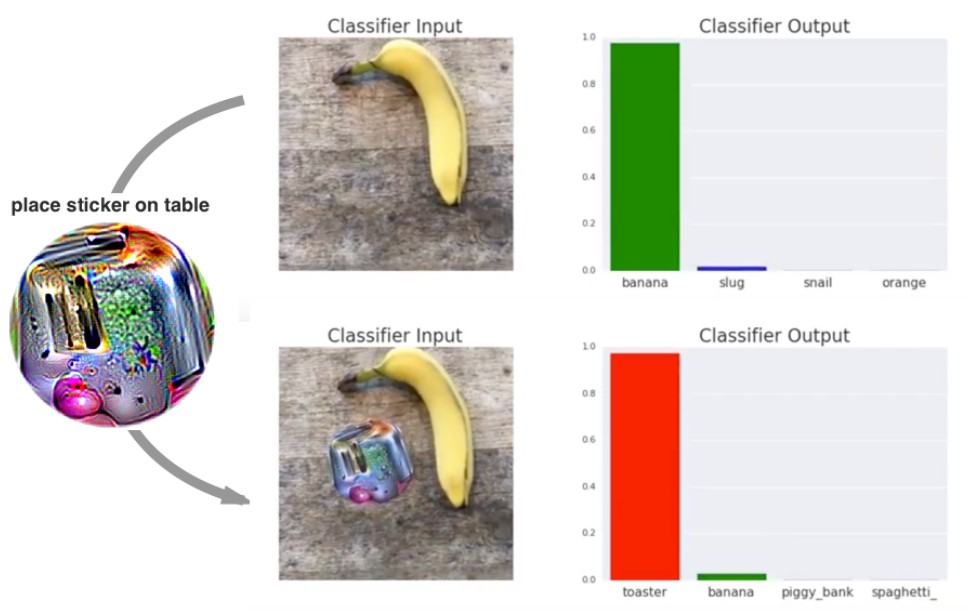
\includegraphics[scale=0.5]{figures/chapter_intro/adv_patch.jpg}
\caption{Perceivable perturbations as a patch}
\label{fig.adv_patch}
\end{figure}

A variant of the Expectation over Transformation (EOT) framework \citep{athalye2018synthesizing} is used to obtain the trained patch. In particular, the patch is trained to optimize the objective function:

$$\hat{p} = \arg \underset{p}{\max}\mathbf{E}_{x \sim X, t \sim T,l \sim L}[logPr(\hat{y}|A(p,x,l,t))]$$

where $X$ is a training set of images, $T$ is a distribution over transformations of the patch, and $L$ is a distribution over locations in the image \citep{brown2018adversarial}.

To design a printable physical patch, Non-Printability Score (NPS) can be used for measuring the error between a printed pixel and its digital counterparts. Sum of NPSs of all pixels in an image can be used to measure the image printability \citep{wang2021daedalus}.

$$\hat{p} = \arg \underset{p}{\min}\mathbf{E}_{x \sim X}\mathbf{E}_\phi f_3(x, p, \Phi) + SNPS(p, \beta)$$

where SNPS is the Sub-sampled Non-Printability Score of the poster $p$.

In chapter \ref{chpt:driving}, we introduce real-time white-box attacks against autonomous driving systems that that generate unnoticeable full-image perturbation.

In chapter \ref{chpt:detection}, we present real-time white-box attacks against object detection that generate noticeable adversarial patches.

% \clearpage

\subsection{Black-Box Attacks}
\label{sec:blackbox_attack}

White-box attacks that rely on gradients can generate adversarial inputs in real-time. However, gradients are not computed in real-world deep learning applications because those applications only perform the inference that does not require gradients. Without access to gradients, white-box attacks become infeasible in the real world.

Without access to gradients, black-box attacks generate adversarial inputs via querying. The Zeroth Order Optimization (ZOO) Attack amends the C\&W white-box attacks to the black-box setting by modifying the loss function and computing an approximate gradient using a finite difference method \citep{Chen_2017}.

$$f(x,t) = \max \{ {\underset{i \neq t}{\max}\ log[F(x)]_i - log[F(x)]_t, -\kappa } \}$$

The ZOO Attack relies on the output of confidence scores to estimate the gradient, while decision-based attacks can generate adversarial inputs using even less information.

\begin{figure}[H]
\centering
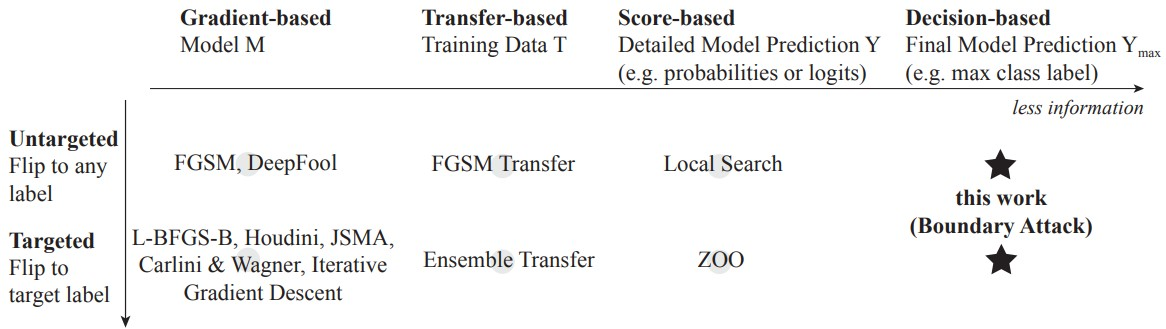
\includegraphics[scale=0.45]{figures/chapter_intro/query-efficient.jpg}
\caption{Decision-based adversarial attacks \citep{brendel2018decisionbased}}
\label{fig.query}
\end{figure}

For image classification tasks, decision-based attacks only require access to the predicted class, while score-based attacks require the predicted probability of each class.

\begin{figure}[H]
\centering
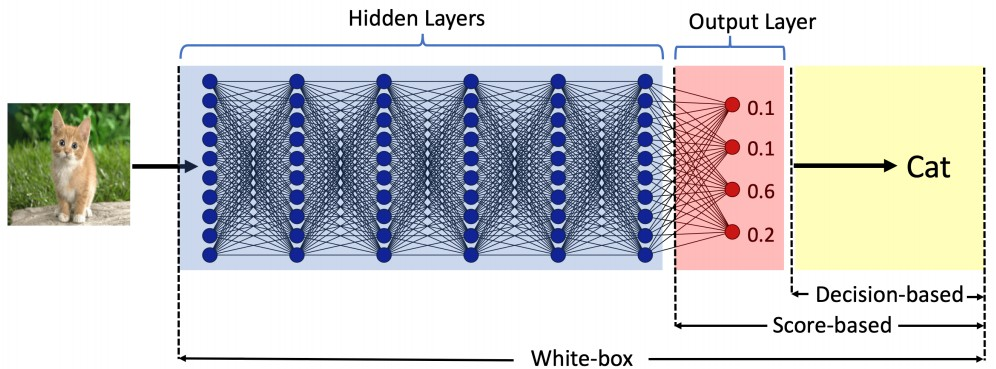
\includegraphics[scale=0.35]{figures/chapter_intro/score-decision.jpg}
\caption{The difference between score-based and decision-based attacks \citep{chen2020hopskipjumpattack}}
\label{fig.decision}
\end{figure}

In chapter \ref{chpt:classification}, we present adversarial classification, a black-box attack against cloud services of image classification.

\section{Research Questions}
\label{sec:research_question}

\section{Thesis Overview}

To achieve the research objectives set out in Section 1.4, the remaining of the thesis organized as follows:

Chapter 2: publication
